The Königsberg bridge problem, which was posed and answered in the negative by Euler in 1736 represents the beginning of graph theory \cite{graph-weisstein}. A \textbf{graph} is a generic data structure and is a super set of lists, and trees. Social networks, co-author networks, citation networks, computer networks, road networks, (artificial) neural networks, and financial networks are are real-life manifestations of graphs. \textbf{Interaction} between messenger molecules in the body, interaction between people on social media, and spreading of infectious diseases, are also modelled as graphs. Finding the shortest \textbf{path} between two points, and \textbf{sorting web pages} in order of importance are also graph problems. Graphs are indeed unifying abstractions that can leverage interconnectedness to represent, predict, and explain several phenomena \cite{graph-sakr21}.
% The \textbf{assignment of registers} to variables (by compiler), and the assignment of \textbf{available channels} to a radio transmitter are also graph problems. 

\textbf{Static graphs} are those which do not change with time. Static graph algorithms are techniques used to solve such a graph problem (developed since the 1940s). Static algorithms are also known as off-line or start-over algorithms \cite{incr-ramalingam96}. To solve problems on larger and larger graphs, a number of optimizations (both algorithmic and hardware/software techniques) have been developed to take advantage of \textbf{vector-processors} (like Cray), \textbf{multicores}, and \textbf{GPUs}. A lot of research had to be done in order to find ways to enhance parallelism. The techniques include a number of \textbf{parallel algorithms}, \textbf{concurrency models}, \textbf{locking techniques}, \textbf{transactions}, etc. This is especially due to a lack of \emph{single-core performance} improvements.

Graphs where relations vary with time, are called \textbf{dynamic graphs}. The updates to these relations can be changes, insertions, or deletions of vertices / edges. Many problems use dynamic graphs. These dynamic graphs can be thought of as a series of static graphs at different points in time. In order to solve graph problems on these dynamic graphs, one possibility is to take the graph at a certain point in time, and run the necessary static graph algorithm on it. However, as the size of the dynamic graph grows, this repeated computation becomes increasingly slower. It is possible to take advantage of previous results, in order to compute the result for the next time point. Such algorithms are called \textbf{dynamic graph algorithms}, or on-line graph algorithms \cite{incr-ramalingam96}.

Interactive systems such as program development, document writing, and computer-aided design (CAD) where the users build and update an object gradually, and the object has to repeatedly processed in some fashion as it is being built up cannot be supported with static algorithms \cite{incr-ramalingam96}. Since the inception of the Internet and the World Wide Web (WWW), the web graph has been growing at an exponential rate. Given that this web graph is being constantly updated, search engines must repeatedly update their rankings of web pages in order to generate relevant (recent) search results. However, the sheer size of the web graph they need to process makes using a static algorithm unacceptable. Applications such as these make the study of parallel dynamic graph algorithms relevant.

A static algorithm $f(\cdot)$ is one which takes in an input graph $x$ and generates an output $y$, as shown in Figure \ref{fig:about-static-vs-dynamic-algorithm}. On the other hand, a dynamic algorithm $g(\cdot)$ accepts the original input $x$, the original output $y$, and importantly the change in input $\Delta x$, and provides us with the updated output $y + \Delta y$ as shown in Figure \ref{fig:about-static-vs-dynamic-algorithm}. It may also accept an additional auxiliary information as input, and generate an output auxiliary information. The objective is to identify the part of the output which is no longer correct, and update it. If it is not possible to exactly determine the part of the affected output, and hence the part of the input that needs to be processed, we should overestimate it \cite{incr-ramalingam96}.

The efficiency of a dynamic algorithm depends on how well that affected part if the output is estimated from the change in input. As long as the change in output is sufficiently small, the actual size of the input should in general not affect the execution required by the algorithm. The efficiency of dynamic algorithms also depends upon the overhead for determining the part of input that needs to be processed. Unlike a static graph algorithm, where the worst-case time complexity (using big-$O$ notation) is expressed in terms of input size parameters, such as $n$ (total number of vertices in the graph) and $m$ (total number of edges in the graph); the time complexity of a dynamic algorithm is expressed in terms of change in input and the associated affected output $\delta$ size, which is usually written as $||\delta||$. It should be noted that there exist unbounded dynamic graph problems, where the worst-case time complexity has to be expressed in terms of the size of original input. Dynamic algorithms for such problems may still perform better than static algorithms, in the average case \cite{incr-ramalingam96}.

\begin{figure}[hbtp]
  \centering  % \vspace{-0.3 cm}
  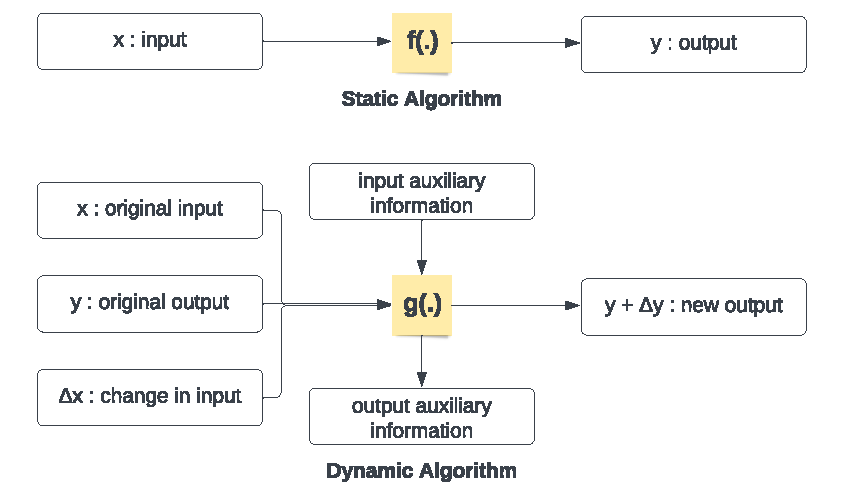
\includegraphics[width=0.70\textwidth]{out/about-static-vs-dynamic-algorithm.pdf}
  \caption{Comparison of a \emph{static} and a \emph{dynamic} algorithm. \cite{incr-ramalingam96}.}
  \label{fig:about-static-vs-dynamic-algorithm}
\end{figure}



A dynamic algorithm can be incremental, decremental, or fully dynamic. Incremental algorithms are those which only consider additions to the initial graph (possibly starting from empty graph), while decremental algorithms only consider only deletions to the initial graph (such as decremental Breadth-First Search or BFS by Shiloach et al. \cite{bfs-shiloach81}). Incremental and decremental algorithms are also collectively known as partially dynamic algorithms. \textbf{Fully dynamic algorithms}, on the other hand, consider both additions and deletions to the graph \cite{graph-italiano99} (such as fully dynamic Transitive closure by King et al. \cite{closure-king08}).

A fully dynamic graph algorithm can accept one or more vertex/edge insertions/deletions. When it accepts a \textbf{batch} (multiple) of insertions and deletions, it is known as a batched fully dynamic graph algorithm. Processing multiple changes to the graph allows the algorithm to amortize the cost of requisite computation on the affected region of the graph, as well as the overhead associated with determining this affected region. The appropriate choice of batch size depends upon frequency and size of updates to the input, and the required frequency of output updates.

The study of parallel dynamic graph algorithms is an ongoing area of research, which includes new algorithms, hardware/software optimization techniques for distributed systems, multicores (shared memory), GPUs, and even FPGAs. Optimization of algorithms can focus on \textbf{space complexity} (memory usage), \textbf{time complexity} (query time), \textbf{preprocessing time}, and even \textbf{accuracy of result}.

% While dynamic algorithms only focus on optimizing the algorithm’s computation time, \textbf{dynamic graph data structures} focus on improving graph update time, and memory usage. Dense graphs are usually represented by an adjacency matrix (bit matrix). Sparse graphs can be represented with variations of adjacency lists (like CSR), and edge lists. Sparse graphs can also be thought of as sparse matrices, and edges of a vertex can be considered a bitset. In fact, a number of graph algorithms can be modeled as \textbf{linear algebra} operations (see \textbf{nvGraph} \footnote{https://github.com/rapidsai/nvgraph}, \textbf{cuGraph} \footnote{https://github.com/rapidsai/cugraph} frameworks). A number of dynamic graph data structures have also been developed to \textbf{improve update speed} (like Packed-Memory Array or PMA), or \textbf{enable concurrent updates} and computation (like \textbf{Aspen's} \footnote{https://github.com/ldhulipala/aspen} compressed functional trees) \cite{graph-besta19}. These data formats are illustrated in Figure \ref{fig:about-graph-representation}.

% \begin{figure*}[hbtp]
  \centering
  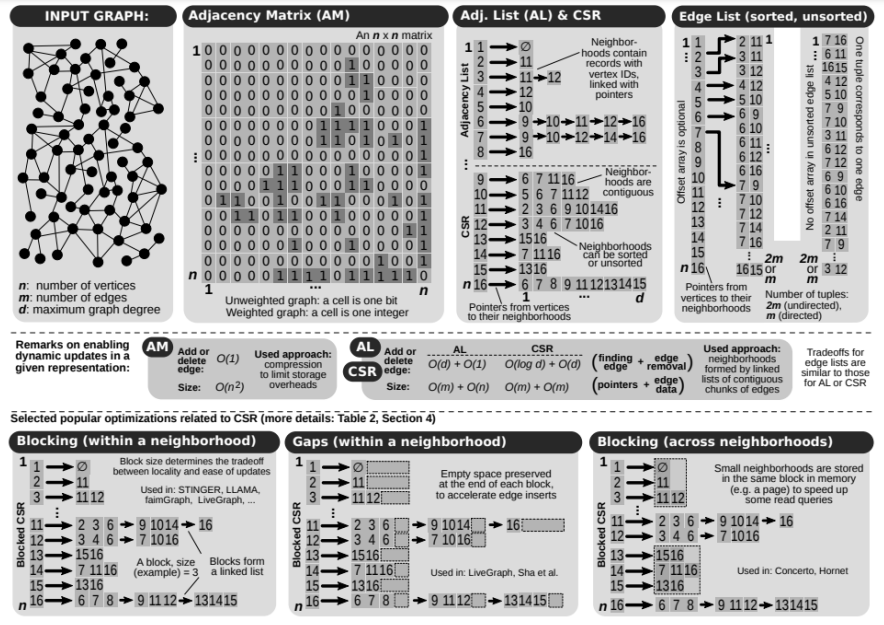
\includegraphics[width=0.98\textwidth]{out/about-graph-representation.png}
  \caption{Illustration of fundamental graph representations (Adjacency Matrix, Adjacency List, Edge List, CSR) \cite{graph-besta19}.}
  \label{fig:about-graph-representation}
\end{figure*}



Streaming / dynamic / time-evolving \textbf{graph data structures} maintain only the latest graph information \cite{graph-besta19}. Streaming graphs can grow indefinitely as new data arrives. They are typically unbounded, thus the underlying systems are unable to keep the entire graph state \cite{graph-sakr21}. \textbf{Historical graphs} on the other hand keep track of all previous states of the graph. Changes to the graphs can be thought of as \textbf{edge insertions}, \textbf{deletions}, or \textbf{updates}, which are sometimes done in batches. Insertions and deletions on streaming graphs are considered as arrivals and removals from a sliding window \cite{graph-sakr21}. Except for functional techniques, updating a graph usually involves modifying a \textbf{shared structure} using some kind of fine-grained synchronization. It might also be possible to store additional information along with vertices/edges, though this is usually not the focus of research (graph databases allow storage of associated data and labels).

In conclusion, we are in the midst of an unprecedented growth of interconnected data, and graph processing systems are expected to play a vital role. These systems rely on complex runtimes that combine software and hardware platforms, which make fair performance measurement and benchmarking difficult. There is a lack of a widely used performance metric other than response time \cite{graph-sakr21}. We intend to focus on the \textbf{design and implementation of dynamic and streaming graph algorithms in the parallel and the distributed setting}, while following suitable approaches for measuring performance and comparing across alternative methods.




% Figure \ref{fig:about-graph-processing} illustrates a complex pipeline for graph processing.
% \begin{figure}[hbtp]
  \centering
  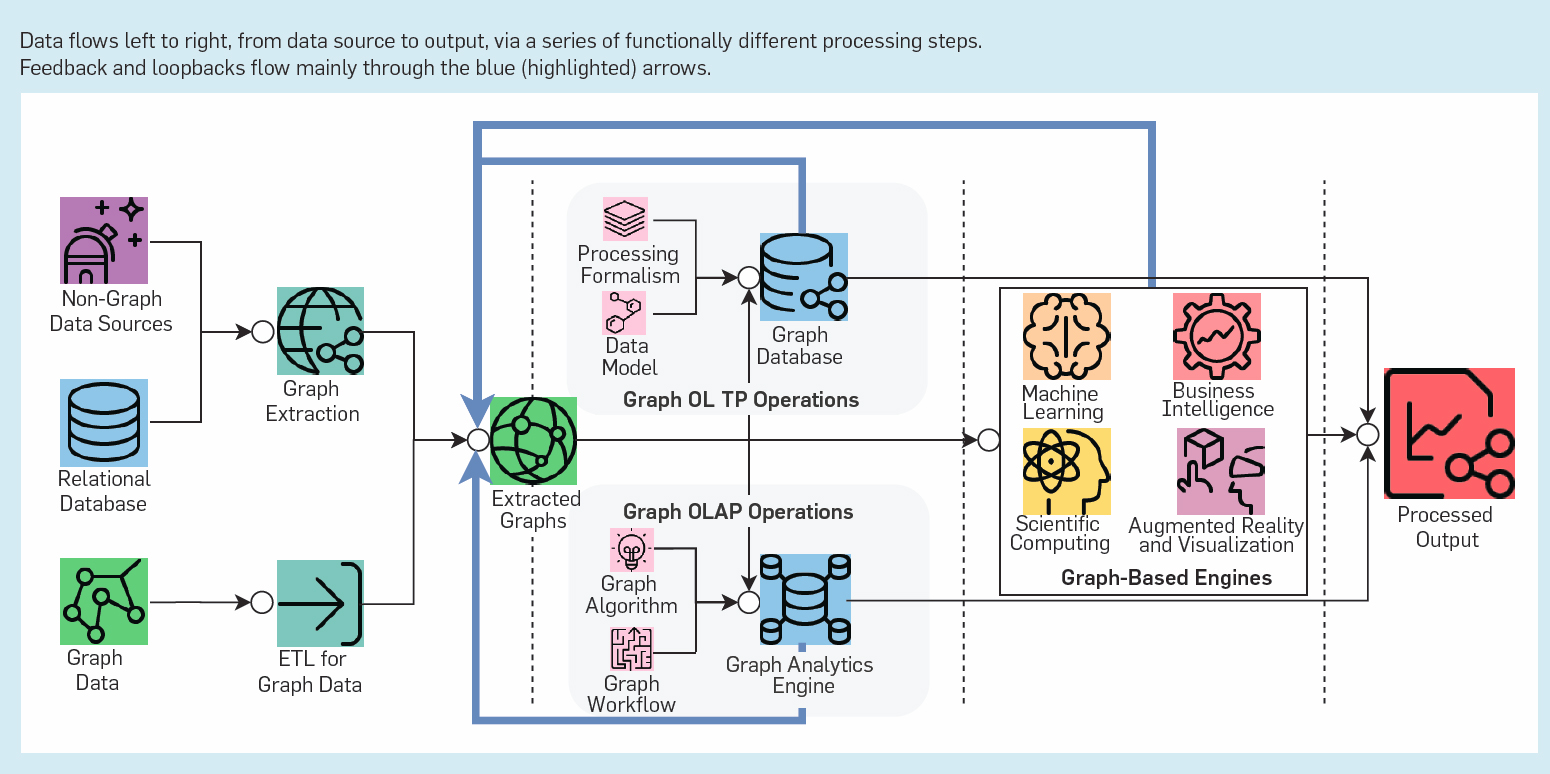
\includegraphics[width=0.98\textwidth]{out/about-graph-processing.jpg}
  \caption{Illustration of a complex data pipeline for graph processing \cite{graph-sakr21}.}
  \label{fig:about-graph-processing}
\end{figure}


% In the recent decade or so, a number of \textbf{graph streaming frameworks} have been developed, each with a certain focus area, and targeting a certain platform (distributed system / multiprocessor / GPU / FPGA / ASIC). Such frameworks focus on designing an improved dynamic graph data structure, and define a fundamental model of computation. For \textbf{GPUs}, the following frameworks exist: \textbf{cuSTINGER}, \textbf{aimGraph}, \textbf{faimGraph} \footnote{https://github.com/GPUPeople/faimGraph}, \textbf{Hornet} \footnote{https://github.com/hornet-gt/hornet}, \textbf{EvoGraph} \footnote{https://github.com/chan150/EvoGraph}, and \textbf{GPMA} \footnote{https://github.com/desert0616/gpma\_demo} \cite{graph-besta19}.
% In conclusion, we are in the midst of an unprecedented growth of interconnected data, and graph processing systems are expected to play a vital role. Figure \ref{fig:about-graph-processing} illustrates a complex pipeline for graph processing. However, the following challenges come up in the design of big graph processing systems \cite{graph-sakr21}:
% \begin{itemize}[itemsep=-1.5em,topsep=0em]
% \item These systems rely on complex runtimes that combine software and hardware platforms, which make fair performance measurement and benchmarking difficult. There is a lack of a widely used performance metric other than response time.
% \item There is considerable tension between performance-oriented specialized graph processing stacks, and productivity-oriented ones that support portability and interoperability. More than 100 big graph processing systems exist, but they do not support portability.
% \item Comprehensive large-scale graph processing experiments lack tractability due to the inability to implement, deploy, and experiment within a reasonable amount of time and cost.
% \item Users have to choose from a large spectrum of graph data models that are similar but differ in terms of expressiveness, cost, and intended use for querying and analytics.
% \item No standard graph library or query language currently exists. However, the Graph Query Language (GQL) standardization project is in progress.
% \end{itemize}
